% Chapter 4

\chapter{Milestones} % 4th chapter title

\label{Chapter4} % For referencing the chapter elsewhere, use \ref{Chapter4} 

\begin{figure}[H]
    \centering
    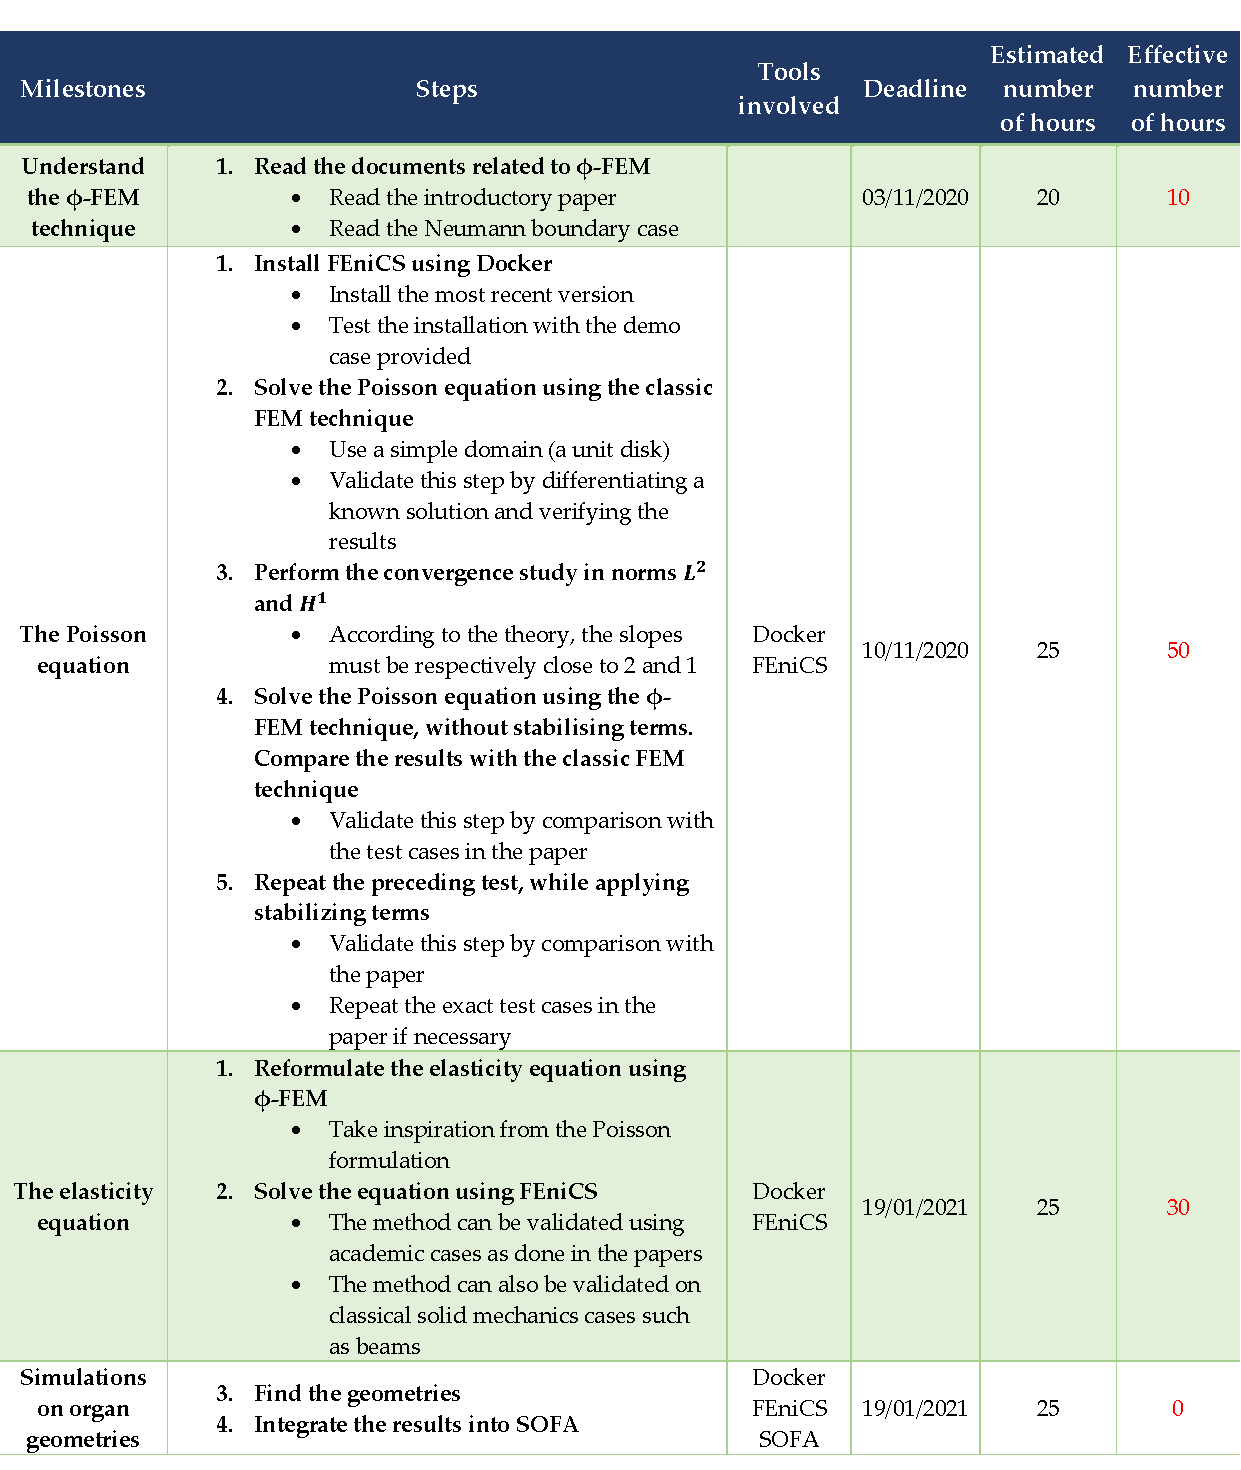
\includegraphics[width=.92\textwidth]{Milestones.pdf}
\end{figure}

The page above summarizes the most important steps we completed, along with their deadlines, the tools needed, the estimated/effective number of hours spent on each objective. We will now be presenting a more detailed report on the conduct of the project, week after week. Each week amounts to at least 8 hours of work ; the early ones were the most consuming. 


\begin{itemize}
    \item[$\blacksquare$] \textbf{Week \#1} - (14/10/2020 - 21/10/2020) : \begin{itemize}
        \item Install the most recent version of FEniCS through Docker.
        \item Then test the installation by solving the Poisson problem using the classic FEM formulation.
        \item Afterwards, perform a convergence study.
        \item Begin reading the paper\footnote{The document known as "the paper" is the main publication describing \phifem (\cite{Reference3}).}.
    \end{itemize}  
    \item[$\blacksquare$] \textbf{Weeks \#2 and \#3} - (21/10/2020 - 03/11/2020) : The required work was to solve the Poisson problem, now using the \phifem  formulation:\begin{itemize}
        \item First without stabilizing terms ;
        \item Then with stabilizing terms.
    \end{itemize}
    \item[$\blacksquare$] \textbf{Week \#4} - (3/11/2020 - 10/11/2020) : Following the unconvincing results from the previous week, \begin{itemize}
        \item Verify that the correct cells are being selected when performing \phifem.
        \item Perform the first test case from the paper, using Sympy.
        \item Finish reading the paper.
    \end{itemize} 
    \item[$\blacksquare$] \textbf{Week \#5} - (10/11/2020 - 17/11/2020) : \begin{itemize}
        \item Put more details about CutFEM and XFEM in the report version 0.
        \item Correct the code for the Poisson PhiFEM.
    \end{itemize} 
    \item[$\blacksquare$] \textbf{Week \#6} - (17/11/2020 - 24/11/2020) : \begin{itemize}
        \item Implement the elasticity equation in classic FEM.
        \item Start the Elasticity equation's implementation in \phifem  by writing the variational form.
        \item Finish wrting the report version 0.
    \end{itemize} 
    \item[$\blacksquare$] \textbf{Week \#7} - (24/11/2020 - 01/12/2020) : \begin{itemize}
        \item Perform a test case with the boundary clamped.
        \item Add convergence details in the report version 0.
    \end{itemize} 
    \item[$\blacksquare$] \textbf{Week \#8} - (01/12/2020 - 08/12/2020) : \begin{itemize}
        \item Finish the elasticity equation's \phifem implementation.
    \end{itemize} 
    \item[$\blacksquare$] \textbf{Week \#9} - (08/12/2020 - 15/12/2020) : \begin{itemize}
        \item Correct the bug in the convergence study.   
        \item Add boundary terms to the formulation.
    \end{itemize} 
    \item[$\blacksquare$] \textbf{Weeks \#10 to \#13} - (15/12/2020 - 12/01/2021) : No additional work was done in this time period.
    \item[$\blacksquare$] \textbf{Week \#14} - (12/01/2021 - 19/01/2021) : \begin{itemize}
        \item Write the report version 1.   
        \item Prepare the slides for the presentation.
    \end{itemize}
    \item[$\blacksquare$] \textbf{Week \#15} - (19/01/2021 - 27/01/2021) : \begin{itemize}
        \item Add corrections for the report version 2. 
        \item Polish the slides.  
    \end{itemize}
\end{itemize}
